% !TEX root = main.tex

\chapter{Experimental results}
\label{ch:results}
This chapter collects all the experimental results obtained during the thesis:
\begin{itemize}
\item Section \ref{sec:resultaod} contains the characterization of the AOD.
\item In section \ref{sec:fullsetup} we characterized different parts of the setup in a test assembly. Polarization, stability, and focus spot have been checked. In particular, two methods have been used to measure a $\mu$m focus spot: razor blade scans, and small pixel size camera.
\item In section \ref{sec:finalsetup}, we performed two experiments with trapped ions: single-qubit manipulation has been demonstrated by performing Ramsey interferometry measurements, which also allowed for a check of addressing performance. Second, a cQED experiment has been carried out, single photons were generated from a single ion in a string, via a cavity-mediated Raman process (Sec. \ref{sec:ramanprocess}).
\end{itemize}
\section{AOD}
\label{sec:resultaod}
The AOD is the core element of the setup, it is therefore essential to characterize it. The two main parameters we are interested in the diffraction efficiency and the response time. For the diffraction efficiency we measure the total output power of the light $P_{tot}$ and then the power of the first diffracted order $P_{1}$. Diffraction efficiency is defined as the ratio between the two.
\begin{equation}
\text{DE} = \frac{P_1}{P_{tot}}.
\end{equation}
Before measuring the diffraction, the optimal RF power to drive the AOD has been found. This was done by maximizing the power of the first diffracted order with the AOD set at its central frequency. Power measurements of the light were done with a Thorlabs PM100D, and the AOD was driven with an amplifier and a RF signal generator. The optimal RF power was found to be 0.11 W, and for the rest of the measurements it was kept at that value. Furthermore, to optimize the linear input polarization, a PBS followed by a half-waveplate were placed before the AOD, the waveplate was rotate trying to maximize the power of the diffracted light. In figure \ref{DE} the plot of the diffraction efficiency as a function of the RF frequency is displayed. Within a bandwidth of 50 MHz from 105 MHz to 155 MHz, we can see that more than 70 \% of the light is in the first diffracted order as expected from the datasheet (Appendix \ref{sec:aoddata}), even though the bandwidth looks shifted with respected to the nominal central frequency of 120 MHz.\\
The response time is the responding time of the light to a RF frequency change. In order to perform this measurement, a voltage controlled oscillator (VCO) was used to generate the RF signal. The VCO was supplied a square wave that alternated between two voltages corresponding to two different frequencies $\sim 96 \to 127$ MHz. The blue light was measured with a photodiode. The photodiode was aligned with the light at one particular frequency, such that when the light moves, the beam would not hit the diode and the signal generated changes. In figure \ref{response}, the signal of the photodiode, together with the supplied VCO signal are plotted. Response time is $\sim 8\,\mu$s, with $3\,\mu$s delay and $5\,\mu$s response. From the beam diameter (13.5 \%) we expect 3.3 $\mu$s response time, while the delay indicates that the distance between the piezo and the edge of the beam is 1.95 mm.

\begin{figure}
\centering
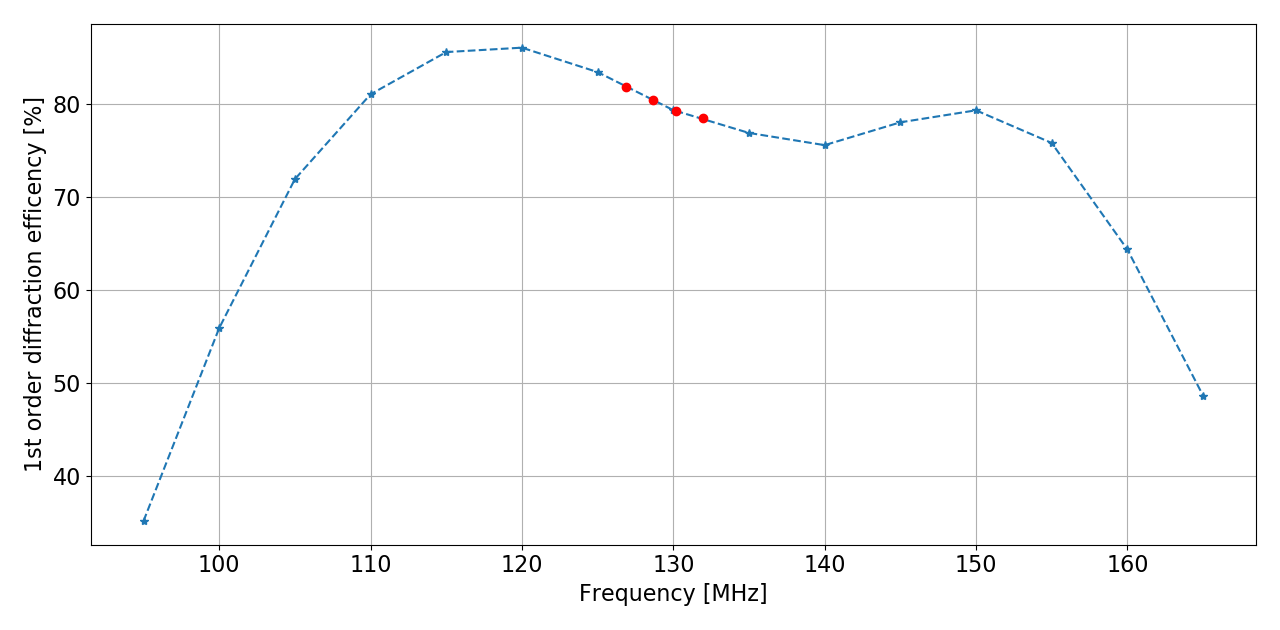
\includegraphics[width = .95\textwidth]{DE2}
\caption{Diffraction efficiency of the AOD as a function of the RF driving frequency. Red points indicate the frequency associated with 4 ions loaded in the trap with a axial COM frequency of 780 kHz as the experiment in section \ref{sec:expqubit}, the theoretical separations are 5.15 $\mu$m for the two outer ones, and 4.77 $\mu$m for the inner ions.}
\label{DE}
\end{figure}

\begin{figure}
\centering
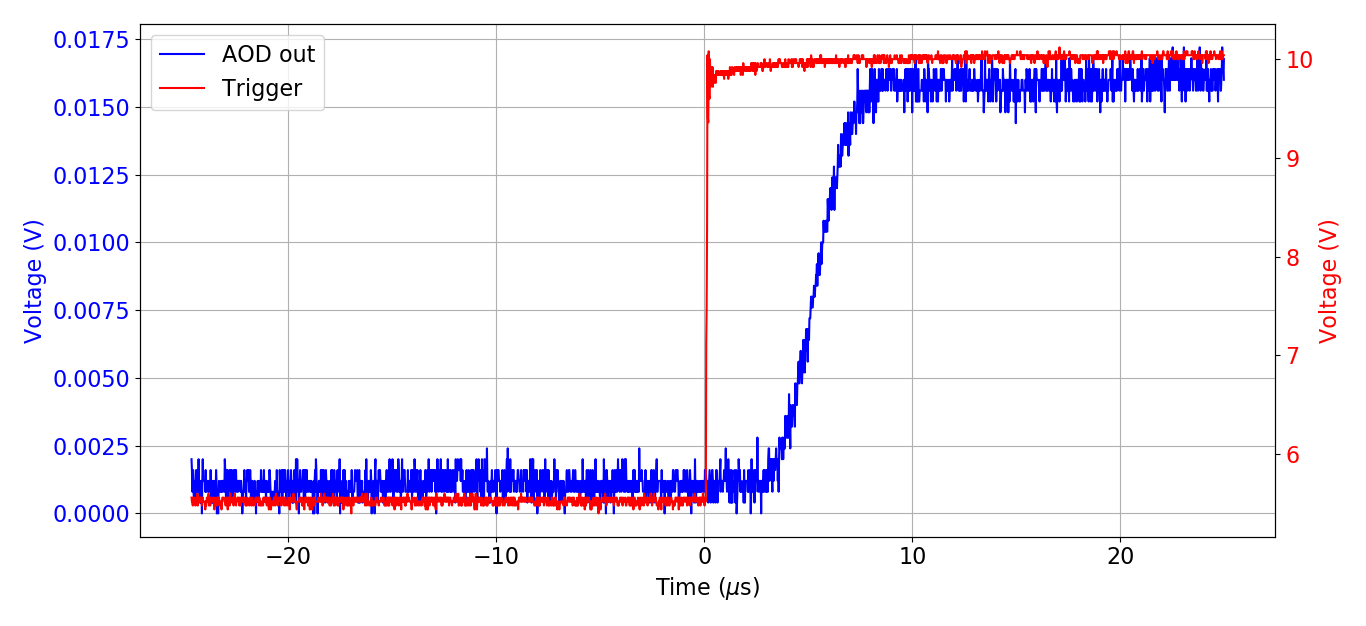
\includegraphics[width = .95\textwidth]{response}
\caption{Response time of the AOD, plotted are the photodiode signal in blue on the left $y$ axis, and the VCO voltage is in red on the right axis. The voltage of the VCO determines the frequency of the RF sent to the AOD. The change here corresponds to a frequency shift of $\sim$31 MHz.}
\label{response}
\end{figure}

\section{Full test setup characterization}
\label{sec:fullsetup}
The test setup was built on an optical table with a spare objective since the one installed in the vacuum chamber was already in use for ion imaging. The layout of the system in figure \ref{addressingsetup} was replicated.

\subsection{Waist: Knife-Edge method}
\label{sec:knifeedge}
\begin{figure}[H]
\centering
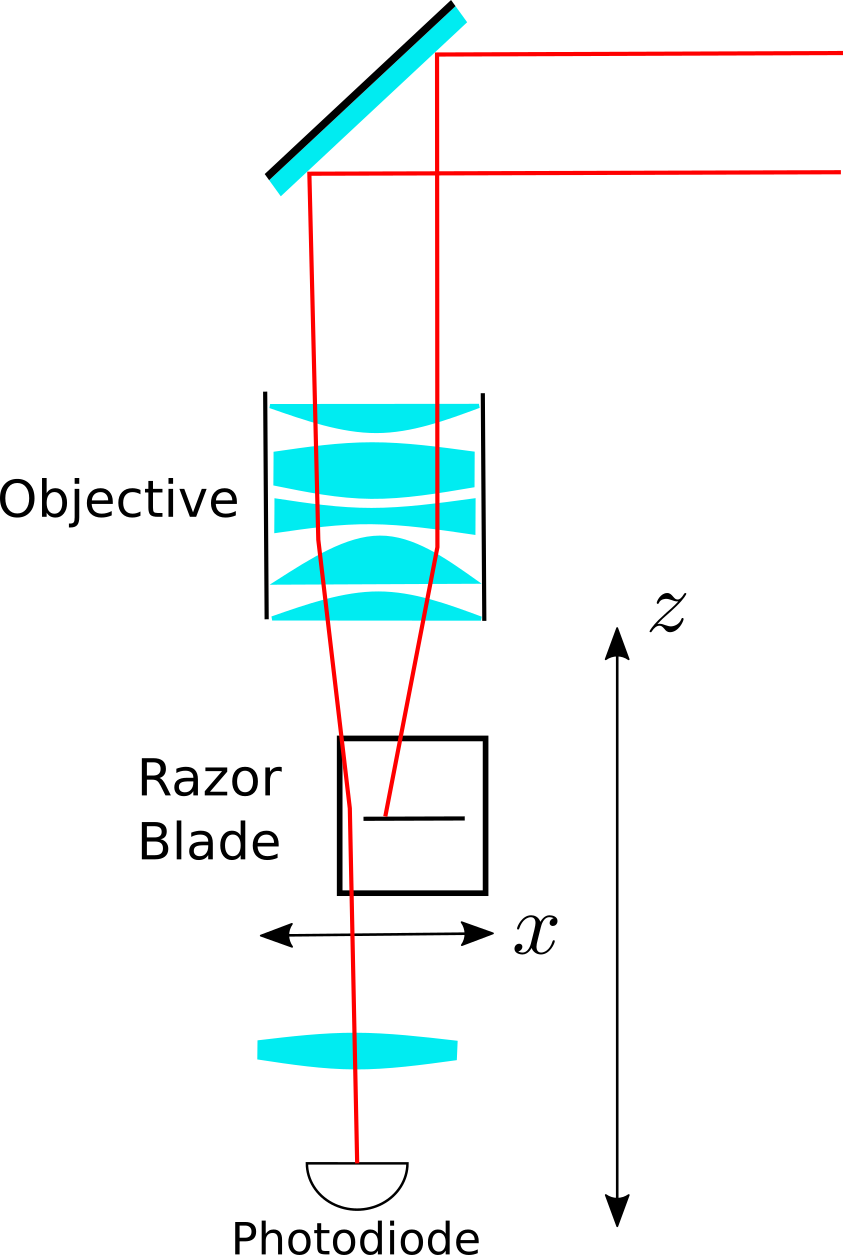
\includegraphics[scale = 1.1]{razorsetup}
\caption{Scheme of the razor scan. A translation stage allows for moving the blade in the direction x, perpendicular to the beam, and z, along the beam.}
\label{razorscan}
\end{figure}
Measuring a micrometer scale waist is not an easy task, the first method applied consisted of mounting a razor blade on a translational stage. The setup used is showed in figure \ref{razorscan}, after the objective the blade is present, and since the beam is quickly diverging after the focus, a lens is used to refocus the light into a photodiode. The stage is moved in the $x$ direction cutting the beam perpendicularly such that the blade is scanning the beam profile. A filter was inserted in order to not saturate the photodiode.
In the $z$ direction the stage was controlled with a manual screw with resolution of $1\,\mu$m. While in the $x$ direction, the stage had to be moved with sub-micrometer precision, so instead there was a piezo actuator controlled by custom software. The same software also controlled a multimeter that measured the voltage of the photodiode. To get the profile $W(z)$ (equation \eqref{waistprofile}) of the beam, the measurement procedure was as follow
\begin{itemize}
\item Position blade at desired $z$ coordinate
\item Scan beam in $x$ direction with blade
\item Beam width extrapolation
\item Shift $z$ direction
\end{itemize}
The procedure is repeated for sufficient values of $z$ to scan at least few Raylegh ranges. The beam width can be calculated from the scans by fitting the data with equation (2) of \cite{knifeedge}. In figure \ref{examplerazorscan} we report an example of a scan taken at the waist of the beam. The errorbars come from statistical average, every data point is a mean over 5 measurement, and the error is the standard deviation. The fit in this case gave a width $W$ of $3.47\pm 0.06\,\mu$m, the smallest width obtained with this method. It is broader that 1 $\mu$m simulated waist. Furthermore, the profile $W(z)$ was not symmetric and could not be fitted with equation \eqref{waistprofile}. A possible explanation is that this method is not suitable for measuring micrometer waists with a typically commercially-available razor blade, the accuracy is limited by the positioner and the blade roughness. The latter was not known at the few micrometer scale of the beam waist. In comparison, authors of \cite{Cannon:86} have used, instead of a common razor blade, a glass substrate etched with an effective knife-edge features with which they were able to measure a 1 $\mu$m waist.
\begin{figure}
\centering
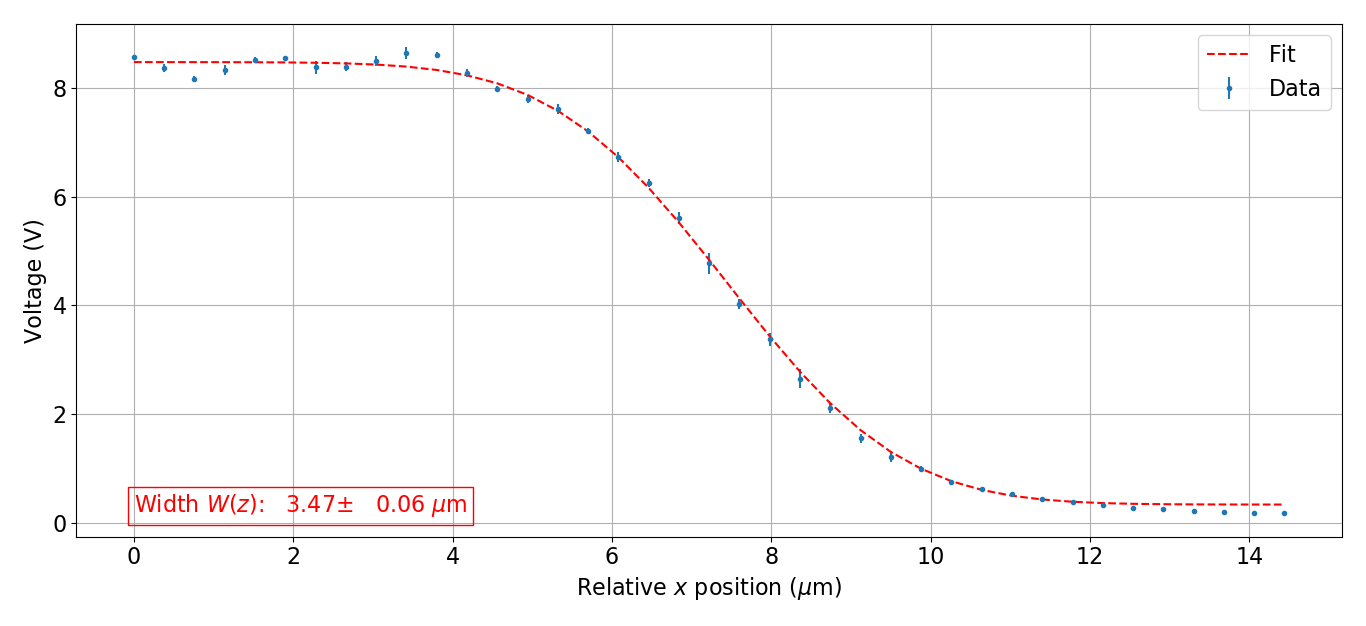
\includegraphics[width=1\textwidth]{img/razorscan}
\caption{Razor scan at the waist of the beam $z=0$}
\label{examplerazorscan}
\end{figure}


\subsection{Waist: Camera}
\label{waistcamera}
Since the Knife-Edge method was not particularly effective, a more direct approach has been subsequently adopted. We measure directly the beam with a camera from IDS model UI-1490LE-M-GL. This particular camera has a pixel size of 1.67 $\mu$m. It should therefore be suitable to measure a focus spot with a $\mu$m precision. A 1$\mu$m focus should hit one single pixel, and if aligned between two pixels, a Gaussian profile could also be fitted.
In addition, unlike the Knife-Edge technique, a camera provides 2-dimensional information about the beam shape and can be exploited to look for aberrations in the system. The setup is almost the same as figure \ref{razorscan}, but the camera now replaces the razor blade, and there is no need for scanning in the $x$ direction, as the $z$ is enough to reconstruct the profile $W(z)$. An additional filter was used to optimize the light reaching the camera in order to not saturate it and get a visible signal.
% \begin{figure}
%      \centering
%      \begin{subfigure}[b]{0.67\textwidth}
%          \centering
%          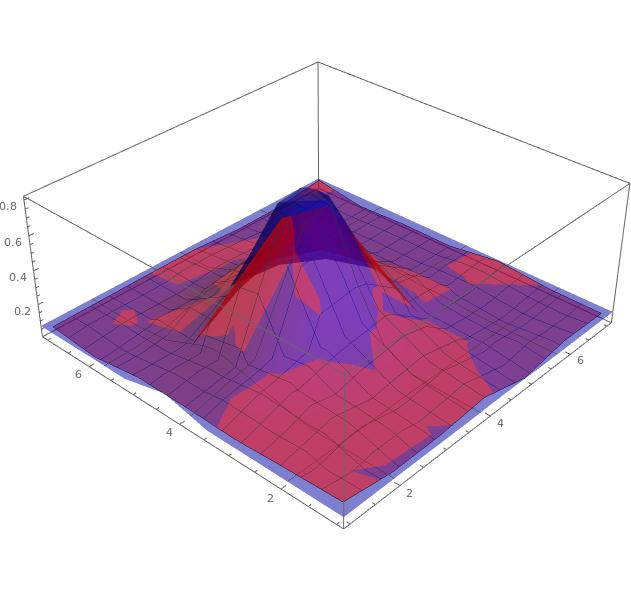
\includegraphics[width = \textwidth]{camera}
%           \caption{Fitted data from the camera. In red color, the normalized pixel value is displayed, while the blue curve is a fitted 2D Gaussian. On the axis there is the pixel number}
%      \end{subfigure}
%      \hfill
%      \begin{subfigure}[b]{0.3\textwidth}
%          \centering
%          
\includegraphics[width=\textwidth]{cameraoriginal}
%         \vspace{5em}
%          \caption{Original photo from the camera.}
%          %\label{fig:three sin x}
%
%      \end{subfigure}
%         \caption{}
%        \label{fig:camera}
% \end{figure}
For every desired $z$ displacement, a photo with the camera is taken, post processed, and then the camera is displaced to the new $z$ coordinate. Post processing is done by fitting the pixel values with a 2-dimensional Gaussian
\begin{equation}
P = A \exp\left\{-\frac{(x-x_0)^2}{2\sigma_x^2}\right\} \exp\left\{-\frac{(y-y_0)^2}{2\sigma_y^2} \right\}.
\end{equation}
The fit parameters are $A,x_0,y_0,\sigma_x,$ and $\sigma_y$. From the standard deviations $\sigma_x$ and $\sigma_y$ the beam width in the $x$ and $y$ direction at position $z$: $W_x(z),W_y(z)$ can be determined as $W_x(z) = 2\cdot 1.67\cdot \sigma_x$ and respectively $W_y(z) = 2\cdot 1.67\cdot \sigma_y$, where $1.67\,\mu$m is the pixel size (see caption of figure \ref{gauss}). The full profiles $W_x(z)$ and $W_{y}(z)$ can be found in figure \ref{cameraprofile}. Here anomalies can be noticed. The profile is asymmetric and does not follow equation \ref{waistprofile}, nonetheless a width $<2.5\,\mu$m has been measured. We decided to install the system and measure more accurately the waist with a single ion.
\begin{figure}
\centering
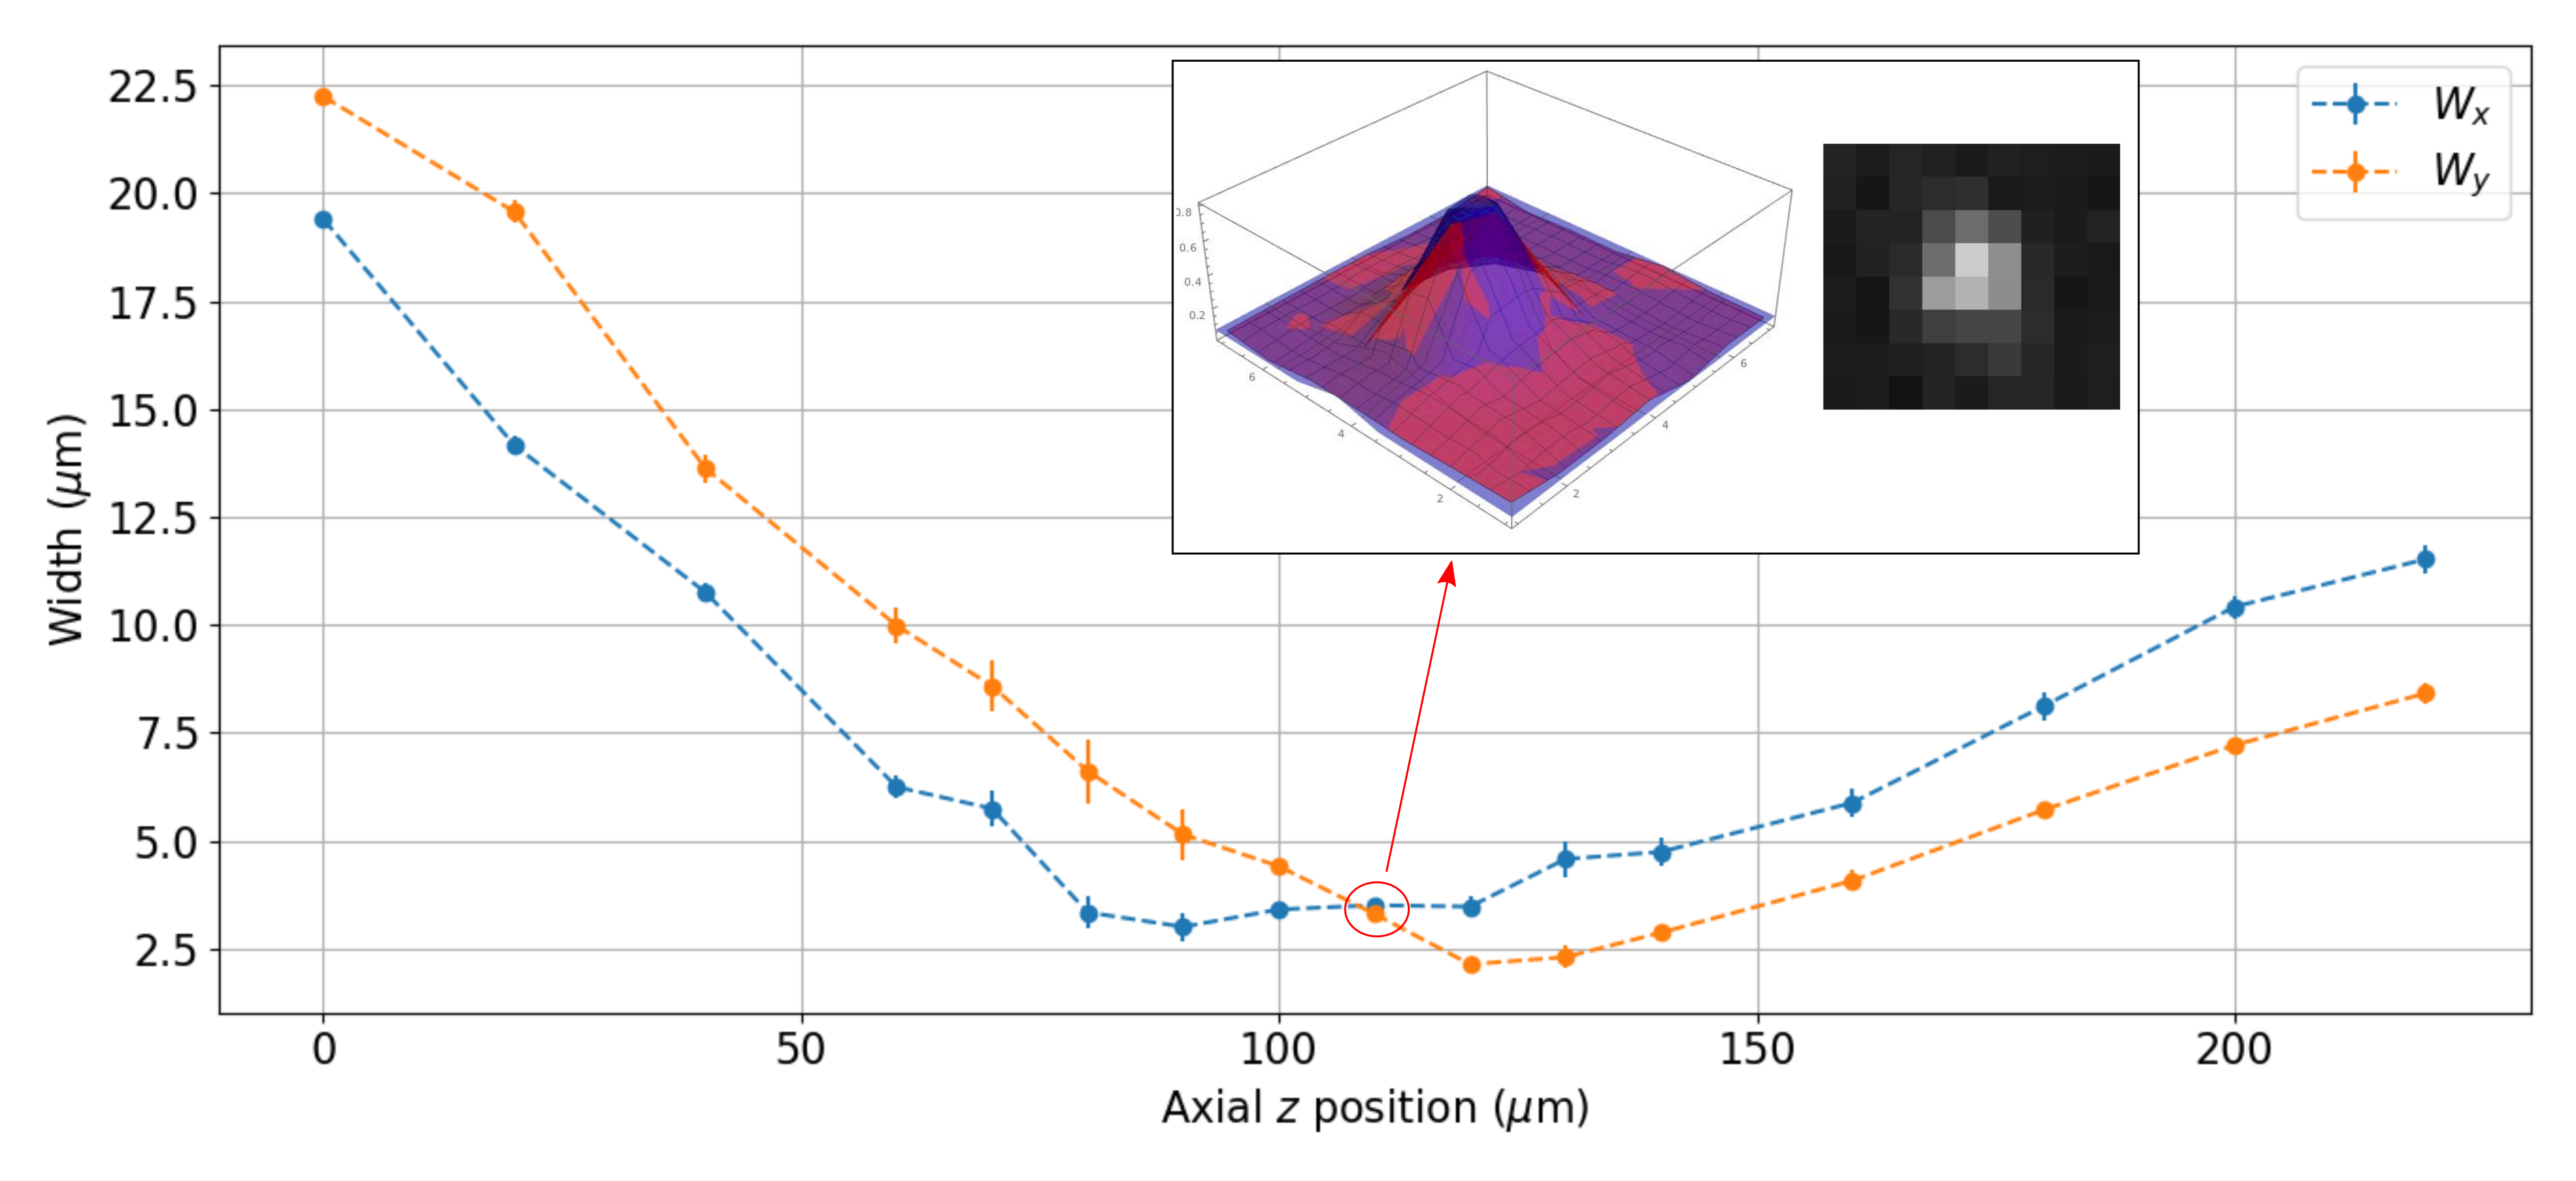
\includegraphics[width=1\textwidth]{cameraprofile_inset}
\caption{Profile of the Gaussian beam along $z$ measured with the camera. Errorbars are estimated from fit. In the inset an example of raw data and Gaussian fit. In red color, the normalized pixel value is displayed, while the blue curve is a fitted 2D Gaussian. On the axis there is the pixel number.}
\label{cameraprofile}
\end{figure}

\subsection{Polarization}
\label{sec:polarization}
As discussed in the design section \ref{sec:addressing} and in the Raman process \ref{sec:ramanprocess}, polarization is an important component as atomic transitions are polarization sensitive, thus the polarization capabilities of the system had to be tested. The goal is to achieve vertical, horizontal, left circular, and right circular polarization at the ion position and test how well they are achieved. Polarization can be changed with two plates: a half wave plate after the AOD, and a quarter wave plate right before the objective, see figure \ref{addressingsetup}. In order to characterize the polarization at various points in the optical path of the addressing setup, the three Stokes parameters $S_i$ \cite{stokes} were measured with a polarimeter from Sc\"after + Kirchhoff series SK010PA.\\
Stokes parameters quantify the type of polarization of an electric field. Linear polarized light has Stokes parameters $S_2,S_3 = 0$, while $S_1 = \pm 1$ for horizontal and vertical polarization respectively. Circular polarized light has $S_1, S_2 = 0$ and $S_3=\pm 1$ for right hand and left hand circular polarization respectively.\\
The first step was to characterize the polarization after the $\lambda/2$ WP B (see figure \ref{addressingsetup}), the main result from this characterization is that horizontal polarization can be achieved immediately after WP B with an angle of $267.2\pm 0.1 ^{\circ}$, and vertical is achieved with an angle of $312.5\pm0.1^{\circ}$ obtained from fitting a sine on the first Stokes parameter. From the same fit, the semiperiod of the polarization is $45.3\pm 0.6^\circ$ consistent with the $45^\circ$ expected for a half waveplate.\\
Afterwards, we measured the polarization after the objective at the focus spot where the ions ideally sit. For this measurement we set the $\lambda/2$ WP B first at $267.2^\circ$, and then at $312.5\pm0.1^{\circ}$, for both numbers we measure the three Stokes parameters as a function of the $\lambda/4$ angle. Results are summarized in table \ref{polarizationstable}, in appendix \ref{app:polarization} the full plots are reported.
\begin{table}
\centering
\begin{tabular}{c c c}
 \toprule
    {Polarization} & {$\lambda/2$ WP B ($^\circ$)} & {$\lambda/4$ ($^\circ$)} \\ \midrule\midrule
   Horizontal & $267.2\pm 0.1$ & $49.7\pm0.1$  \\
   Vertical   & $312.5\pm0.1$ & $48.1\pm0.1$\\ \midrule
   Right circular & $267.2\pm 0.1$ & $4\pm 0.1$ \\
   Right circular & $312.5\pm0.1$ & $93.1\pm0.1$\\\midrule
  Left circular & $267.2\pm 0.1$ & $95.4\pm0.1$\\
    Left circular & $312.5\pm0.1$  & $3.1\pm0.1$\\ \bottomrule
\end{tabular}
\caption{Polarization at the ion position and angles of the waveplates $\lambda/2$ WP B and $\lambda/4$ (Ref. figure \ref{addressingsetup}) that set the polarization. Numbers are found as maxima or minima of a sine fit of the polarization data in appendix \ref{app:polarization}.}
\label{polarizationstable}
\end{table}

\subsection{Stability}
\label{sec:stability}
It is imperative to know the stability of the system in terms of polarization and beam pointing. This means knowing over the course of hours or days if the setup needs to be re-optimized or calibrated. First we measured polarization, it was set to be right circular: $\lambda/2$ set to $267^\circ$, and $\lambda/4$ set to $4^\circ$. We recorded the three Stokes parameters for a total of one hour, this data is plotted in figure \ref{polstability}. It can be seen that the polarization is stable within short term fluctuations over a period of one hour. (check pol error.)\\
Beam pointing stability is the stability of the focus position, which could drift in any direction for any reason. To test it, we recorded the position of the focus for a period of one hour with the camera. The camera was positioned at the focus with the same setup discussed in section \ref{waistcamera}, and then a video was recorded. The video was later analyzed by tracking the the brightest pixel over time. In figure \ref{beampointing} we can see the horizontal $x$ and vertical $y$ position of such pixel. In the horizontal directions, fluctuations of one single pixel can be noticed, which could be a result of the light hitting between two pixels. In the vertical direction the fluctuations are in the order of two pixels, this could indicate that the position might have shifted by one entire pixel over this period. This means that the focus position is stable with an upperbound of $1.6\,\mu$m/hour. We have to consider that this measurement was taken on a open table, a more precise beam pointing stability measurement is carried out with ions in the closed mu-metal shield, see section \ref{sec:singlequbitmanipulation}.

\begin{figure}[H]
\centering
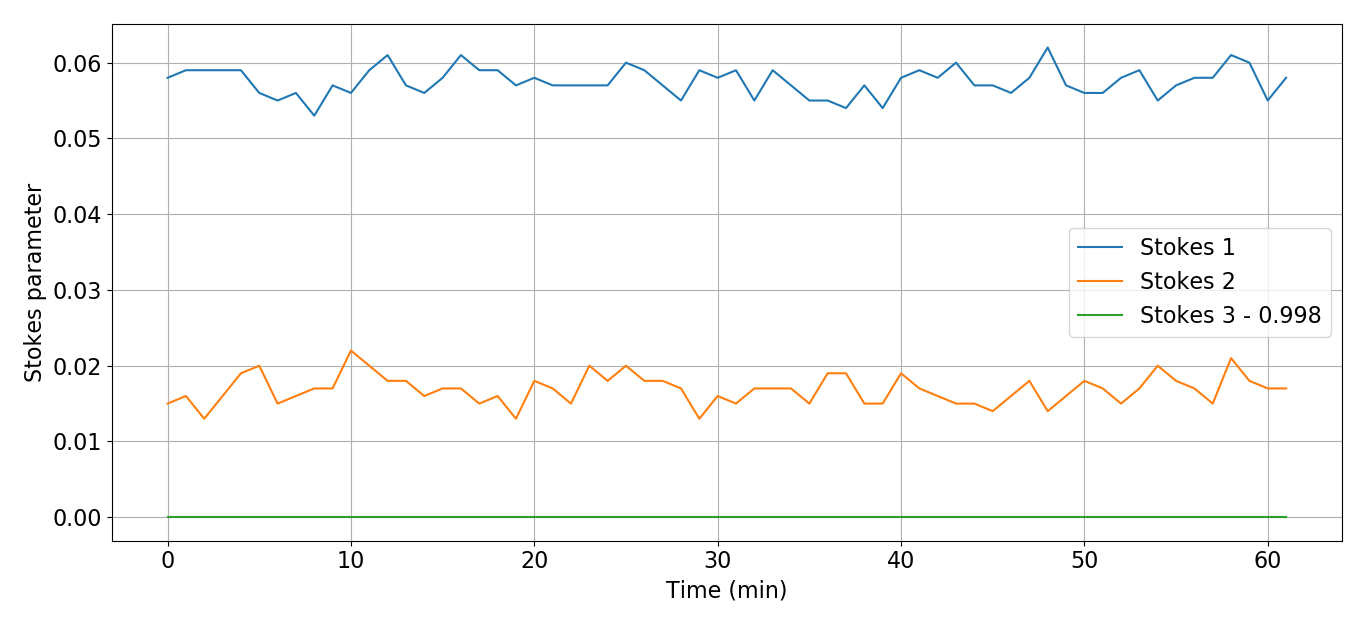
\includegraphics[width = \textwidth]{polstability}
\caption{Right circular polarization stability at the ion position over a period of one hour. To the third parameter $S_3$, 0.998 has been subtracted.}
\label{polstability}
\end{figure}

\begin{figure}[H]
\centering
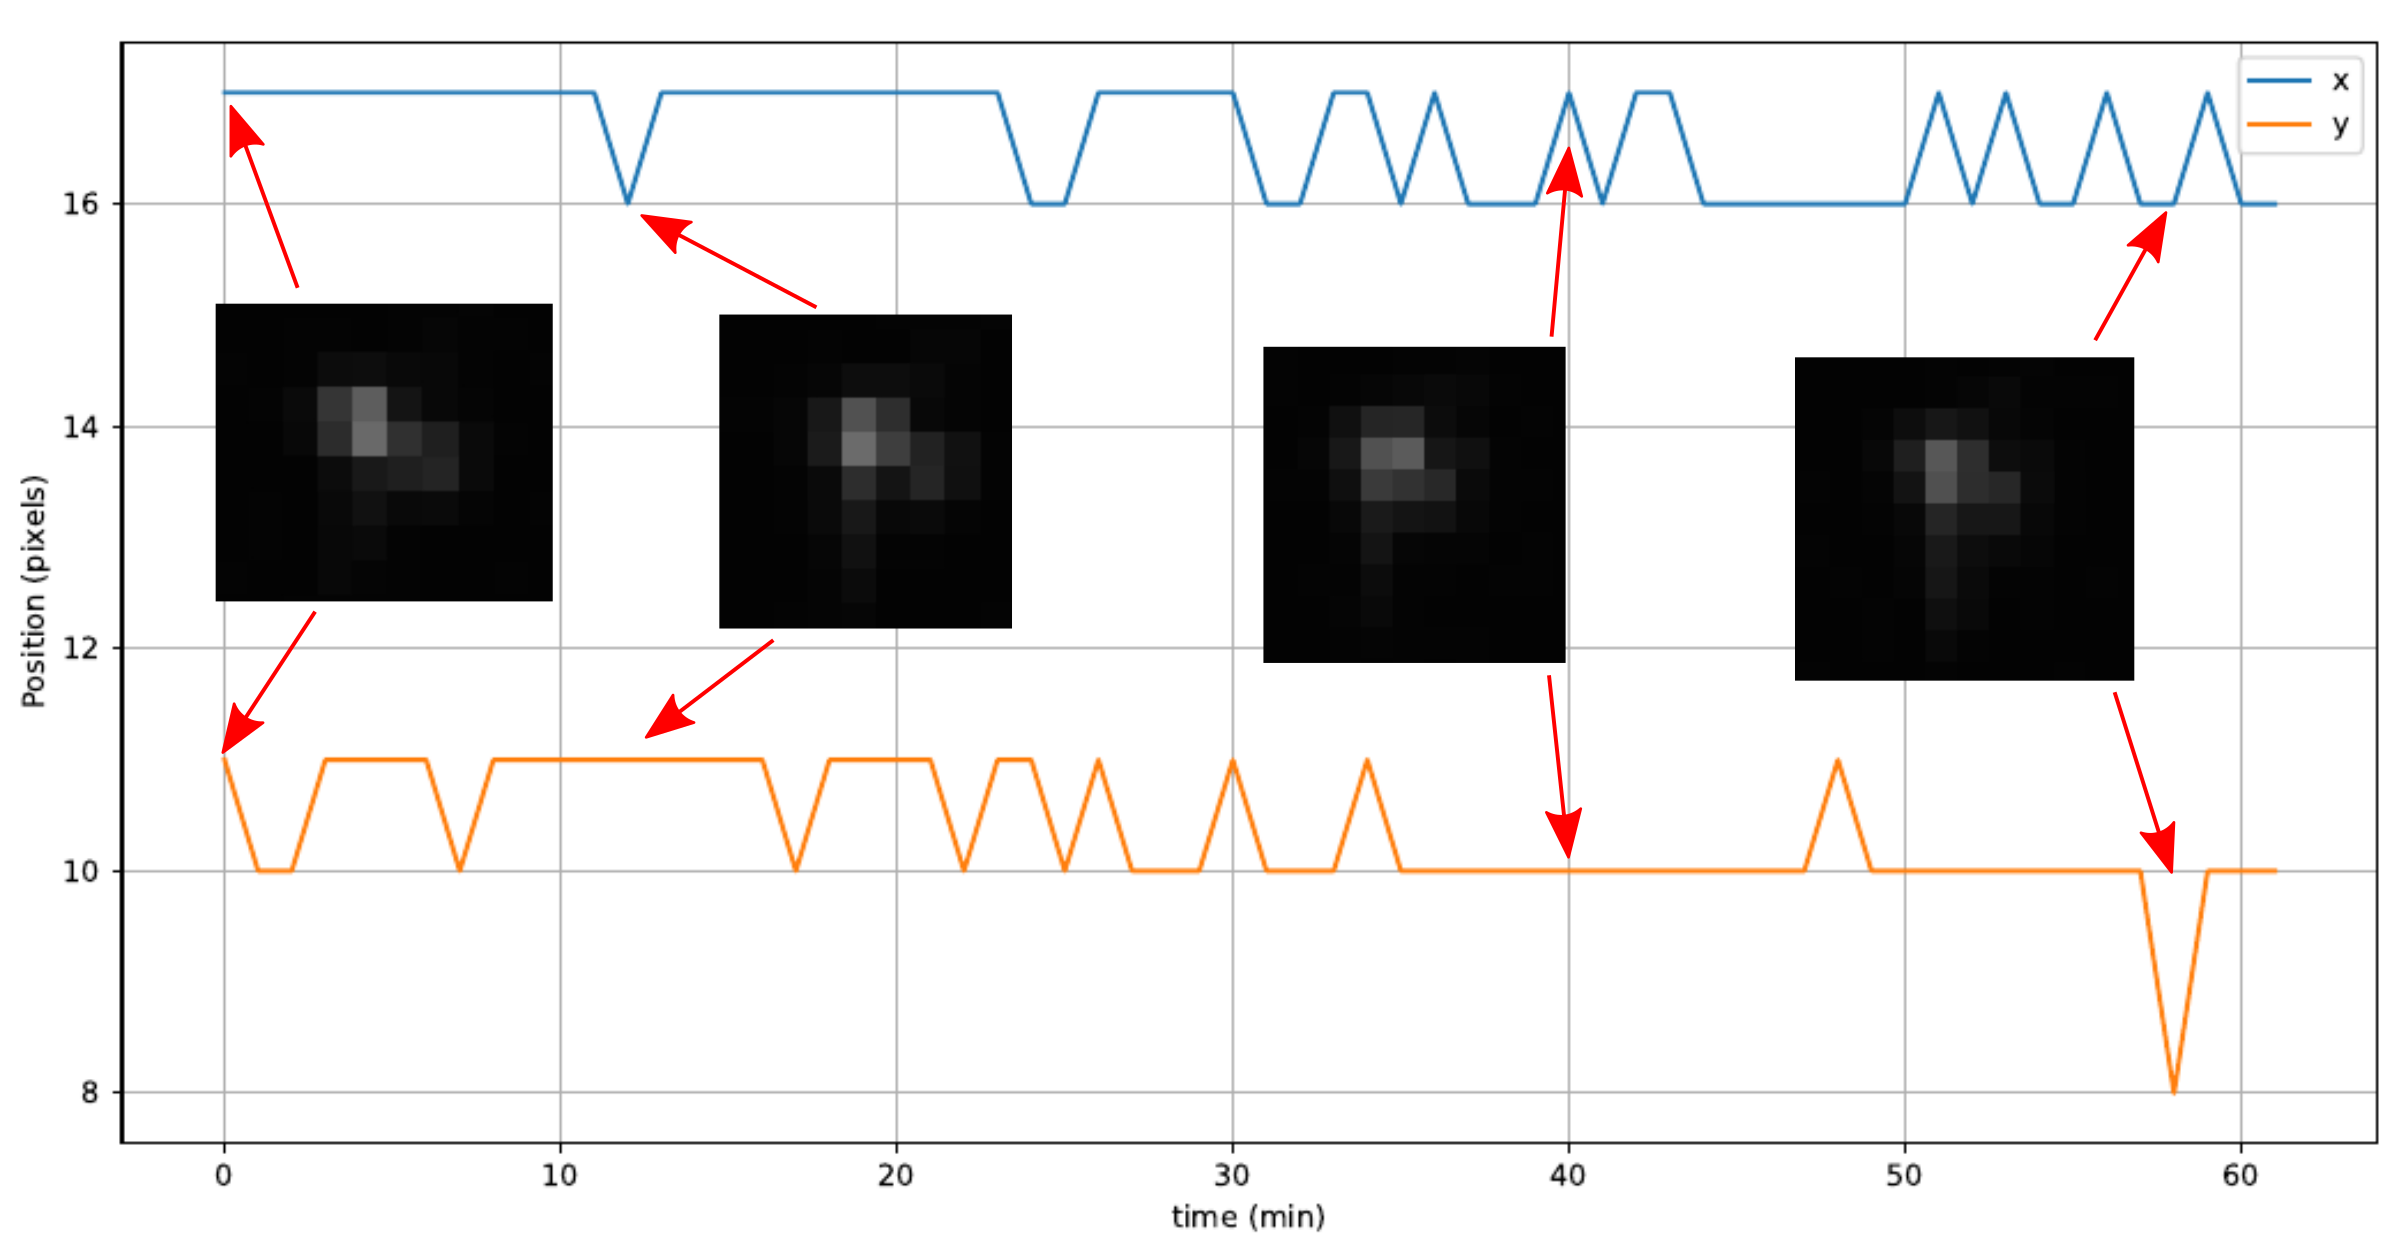
\includegraphics[width = \textwidth]{beampointing2}
\caption{Beam pointing stability at the focus position over a period of one hour. The 2 lines represent the horizontal $x$ and vertical $y$ position of the beam in unit of pixels. In the insets, some examples of raw data are given.}
\label{beampointing}
\end{figure}


\newpage
\section{Final installed system}
\label{sec:finalsetup}
After the tests presented in the previous sections, the setup was installed next to the ion chamber and focused on the ions as described in section \ref{design4}. As there is no more physical access to the focus spot, more advanced quantum optics experiment have to be be carried out in order to measure properties of the system, such as focus spot size and addressing error. The first experiment designed aims exactly at measuring these two quantities: a Ramsey experiment was performed on four loaded ions, from which the beam shape due to AC Stark shifts on the ions could be measured.
The second experiment involves three ions and the goal was to generate photons via Raman process from one single ion leaving the state of the other two unaltered, demonstrating therefore the new possibility to emit single photons from individual ions in a string.

\subsection{Single qubit manipulation}
\label{sec:singlequbitmanipulation}
\begin{figure}[H]
\centering
\includegraphics[width=\textwidth]{sequence}
\caption{Pulse sequence of the experiment. The sequence is repeated for different AOD frequency moving the 393 nm beam across the ion string. From the ion excitations, the Rabi frequency of the 393 nm laser can be inferred.}
\label{sequence}
\end{figure}
The goal of this experiment is to perform the Ramsey experiment discussed in section \ref{sec:expqubit}. In summary, we want to sweep the 393 nm beam along the ions, the sequence in figure \ref{sequence} is repeated for different AOD frequency, and from the ion excitation we can infer Rabi frequency of the 393 nm laser. Before the actual experiment, some preliminary measurements have to be taken, thus in this section we show first the following:
\begin{itemize}
\item Global Rabi flops with 729 nm, from this we can measure the $\pi/2$ pulse time and show individual ion readout with the camera.
\item Ramsey fringes without 393 nm, showing coherent control over the ion qubits.
\item 393 nm pulse length scan, to get the length $\tau$ of the Raman pulse and furthermore to estimate the addressing error.
\end{itemize}
After these preliminary steps we perform the Ramsey experiment scanning the frequency of the AOD, as we scan, every single ion will produce a signal proportional to the Rabi frequency $\Omega$ that can be fitted to obtain the focus spot size.\\
The experiment was done with four ions loaded in the trap with endcap voltages of 714 V and 700V, for which numerical simulations yield a axial COM frequency of $\sim$767 kHz. The 393 nm laser was locked to the wavemeter and detuned by $\sim$3 GHz.\\
Rabi flops are showed in figure \ref{rabiflops4}. Some point are missing in the plot due to a melting event of the ion crystal. The system took the data points while ions were melted, therefore they have been removed. (Why is orange lower?) Rabi flops are also damped due to residual thermal distribution, since we only perform Doppler cooling, ions are not in the ground state, but rather in a thermal state \cite{ross}. The $\pi/2$ time is extrapolated from the first flop as the time it takes for the ions to reach excitation probability $P_D = 0.5$, we estimated 4.2 $\mu$s. Errorbars on the excitation probability have been assigned according to the error on estimating the probability of a binomial distribution \cite{mle}
\begin{equation}
\sigma = \sqrt{\frac{P_{D}(1-P_{D})}{N}},
\end{equation}
where $N = 50$ is the number of repetitions.
\begin{figure}
\centering
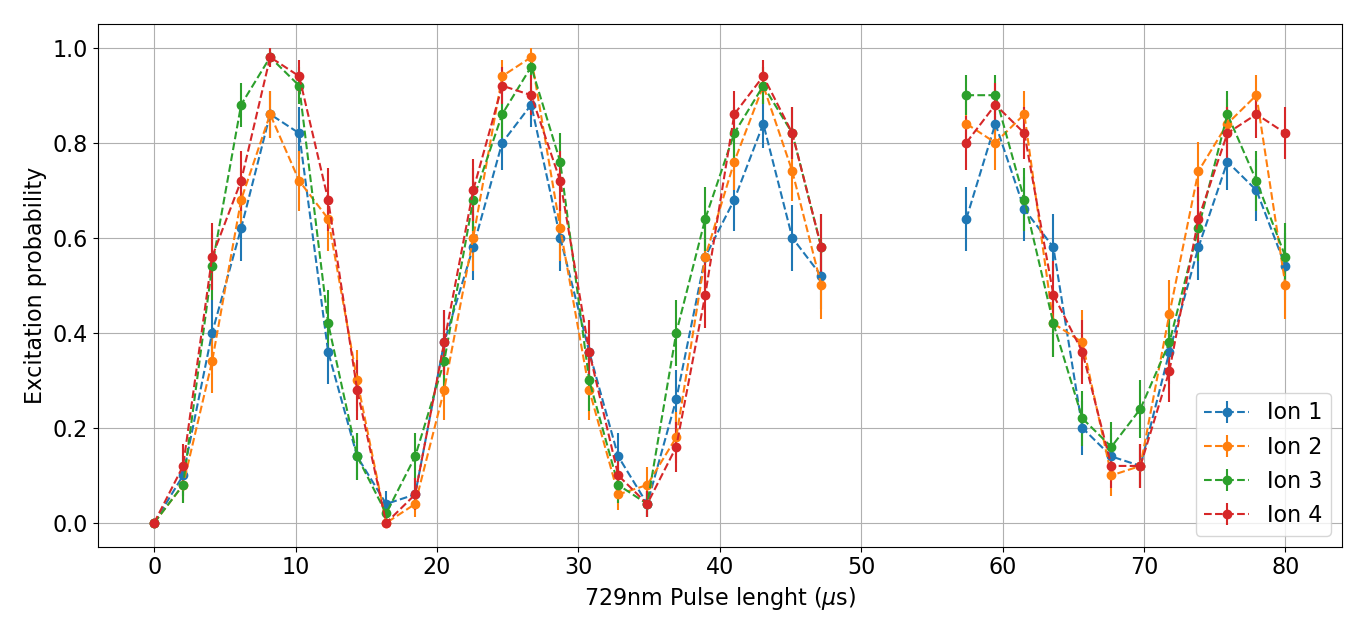
\includegraphics[width=\textwidth]{rabiflops2}
\caption{Global Rabi flops on 4 ions. Errorbars on the excitation probability have been assigned according to the error on estimating the probability of a binomial distribution. Some points were removed due to a melting event.}
\label{rabiflops4}
\end{figure}
Ramsey fringes without the 393 nm pulse are presented in figure \ref{ramseyfringes}, the $\pi/2$ time was set to 4.2 $\mu$s. The phase $\phi$ between the two pulses was scanned, and afterwards it was set to $\phi = \pi/2$ for the rest of the experiment.
\begin{figure}[H]
\centering
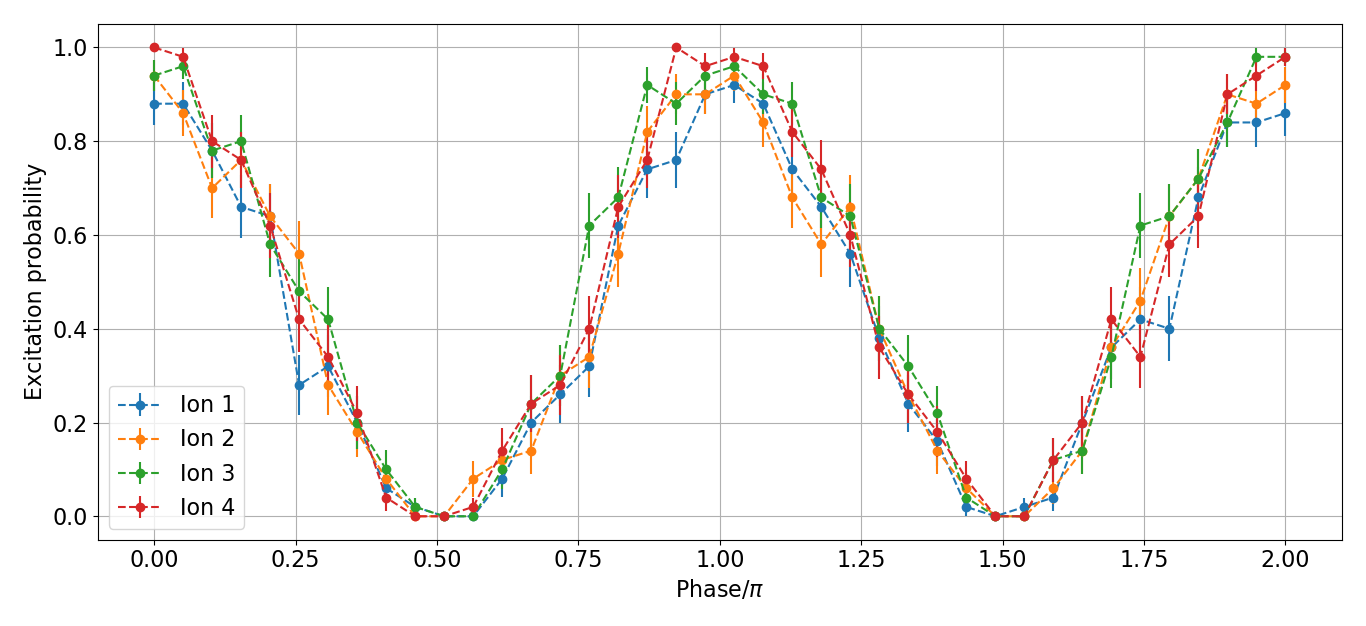
\includegraphics[width=\textwidth]{ramseyfringes}
\caption{Ramsey fringes for 4 ions without 393 nm. A $\cos^2(\phi)$ behavior can be noticed showing coherent control of the ion states.}
\label{ramseyfringes}
\end{figure}
The Raman pulse length $\tau$ was chosen in a way that the shift caused by the 393 nm light does not skip any fringe, i.e. the shift induced by the Raman laser does not flip the ion state. To get this timing, $\tau$ can be scanned and the appropriate value can be estimated, the plot is in figure \ref{ACscan}. We set $\tau$ to be $25\,\mu$s, such that we do not excite the ion more than halfway the fringe.
\begin{figure}[H]
\centering
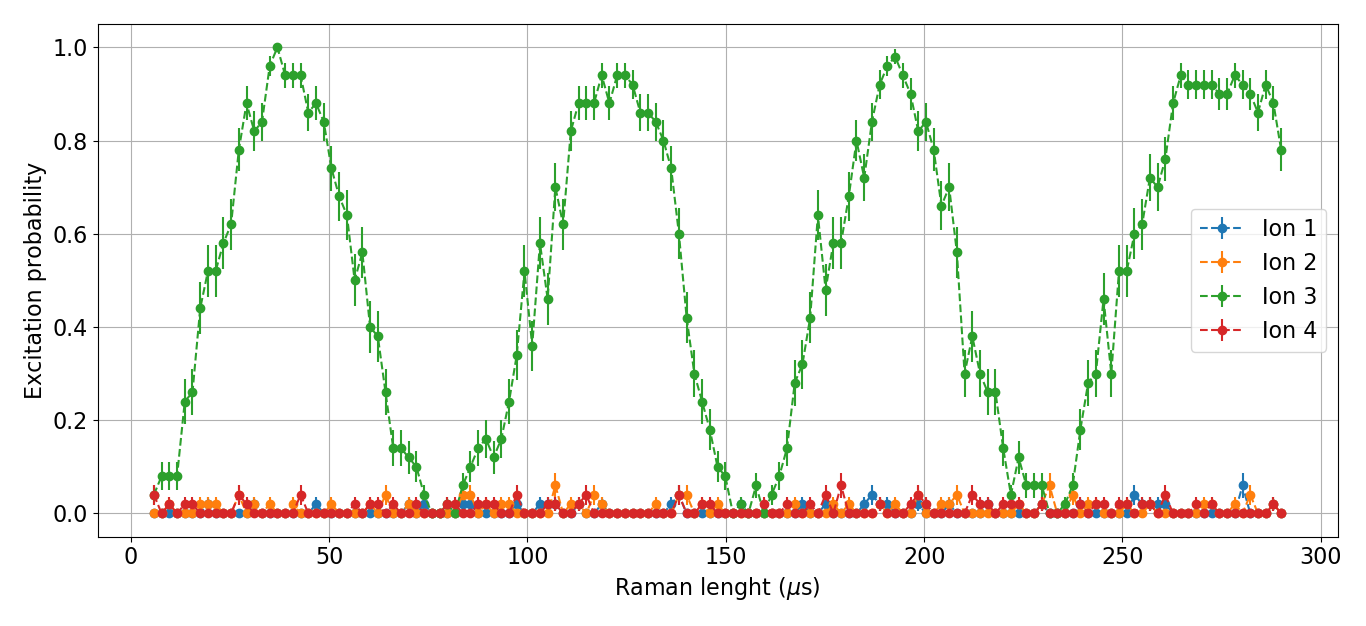
\includegraphics[width=\textwidth]{img/ACscan}
\caption{393 nm AC Stark flops. The pulse length $\tau$ of the 393 nm laser is scanned while shining over one singe ion.}
\label{ACscan}
\end{figure}
Having chosen all the parameters, the experiment can now be performed. The AOD frequency can be now scanned. During this scan the beam is moved from ion to ion and the excitation probability of all ions is measured, this is then translated to Rabi frequency with equation \eqref{eq:ptointensity}. The result after post analysis can be seen in figure \ref{AODscan}. Specifically, the intensity of the beam has been determined from the probability $P_D$ as discussed, errors are propagated accordingly.
\begin{figure}[H]
\centering
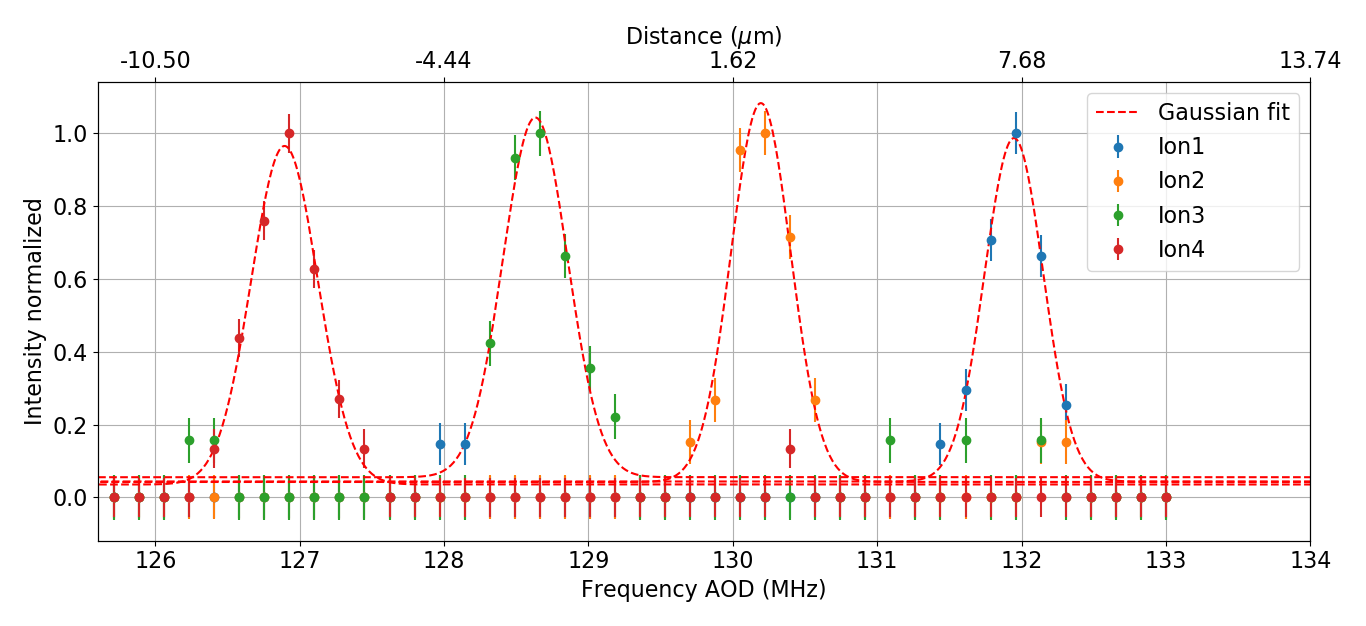
\includegraphics[width=\textwidth]{img/AODScan}
\caption{AOD scanning four ions.}
\label{AODscan}
\end{figure}
To calibrate the beam position scale in micrometers the axial COM mode (767 kHz) of the trap is measured by performing 729 spectroscopy on the carrier and motional sideband. Ions position can be then estimated (cfr. section \ref{ionstrings}. AOD frequencies corresponding to the maxima in figure \ref{AODscan} are attributed to the ion positions, and corresponding frequency shifts to distances. Ultimately, we found a conversion factor of $3.03\,\mu/\text{MHz}$.
The four peaks have been fitted with a Gaussian function to obtain the waist of the beam when focused on the different ions. The waist yielded by the fits from right to left are
$\omega_1 = 1.23\pm 0.20\,\mu$m, $\omega_2 = 1.25\pm 0.19\,\mu$m, $ \omega_3 = 1.35\pm 0.22\,\mu$m, $\omega_4 = 1.39\pm 0.20\,\mu$m.\\
The addressing error can also be estimated from the Stark flops in figure \ref{ACscan}. In this measurement, the addressing beam was focused on one ion and the Raman length $\tau$ is scanned. This increases the interaction time of the laser with the ions, and if the interaction is long enough even the tail of a Gaussian can induce some excitation on the ions on the side of the one being addressed. In the scan displayed, the pulse reached 300 $\mu$s and there is no excitation on any ion apart from the one flopping. Others scans went up to 500 $\mu$s, and still no visual excitation is present. While this means that no quantitative number can be determined for the addressing error, an upper bound can still be given. For an excitation to appear right after 500 $\mu$s, the addressing error should be at most $\Omega_2^2/\Omega_3^2< 10^{-3}$.

\subsection{Photon production}
\label{exp:photons}
The main goal of having an addressed 393nm setup is to generate single photon from individual ion in a chain. In this experiment we produced photons from the central ion of a 3-ions chain by loading a string of 3 ions. A single photon is produced by a pulse of 393nm light focused on the central ion of three via Raman process. In the experiment we scanned the length of this pulse to obtain an integrated wavepacket, i.e. the cumulative probability of detecting a photon as a function of the pulse length. The generated photon is emitted into the cavity, transmitted through the mirror of the cavity, coupled into a fiber, and passes through a PBS before reaching two superconducting nanowire single-photon detector (SNSPD) which clicks if a photon is detected. The detectors have two channels corresponding to two different photon polarizations. Detuning of the Raman laser is essential in this experiment, so one has to take into account the frequency shift induced by the AOD $\sim 127$ MHz. As already briefly mentioned, the shift was compensated with the two AOM's in the 393nm laser setup. The experiment includes an initial stage of Doppler cooling and a final stage of state detection with the camera. Furthermore, the locking light 806nm in the cavity was switched off during the photon generation process, in this time the cavity maintained its position with a sample and hold. The measurement is repeated $N$ times to get the average photon probability and the excitation probability. These two quantities are plotted in figure \ref{probphoton} and \ref{probion}.
\begin{figure}[H]
\centering
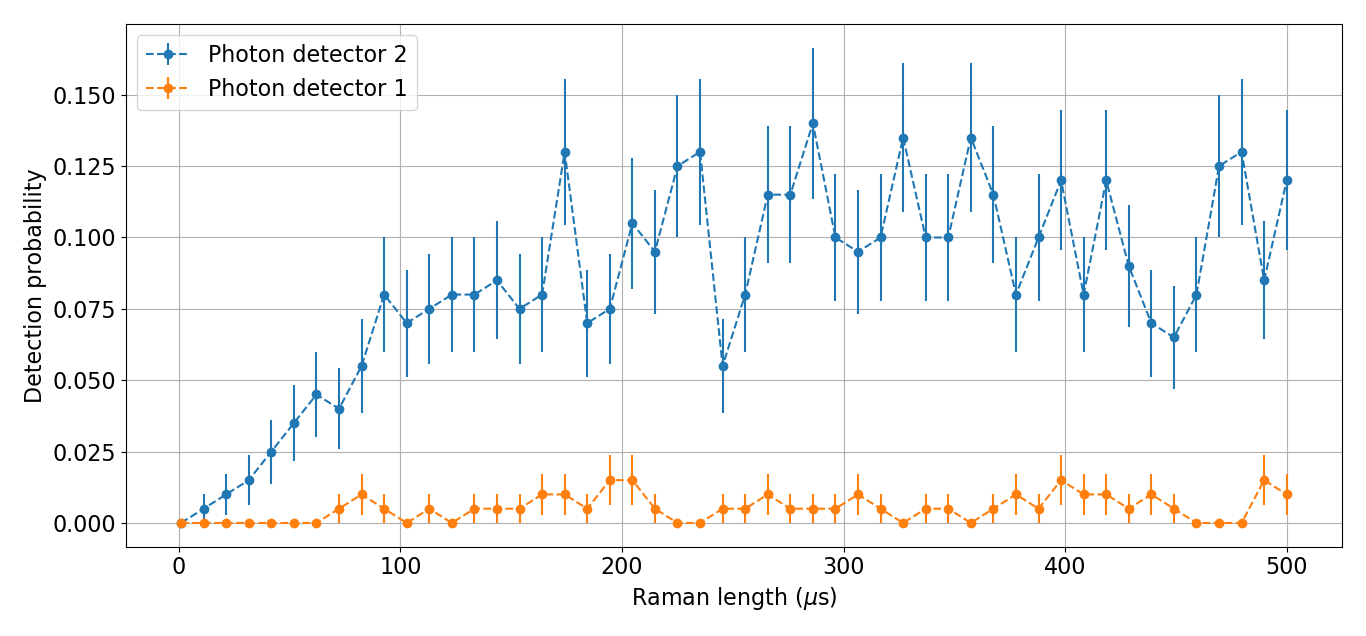
\includegraphics[width=\textwidth]{img/photonefficency_witherror}
\caption{Integrated photon wavepacket. Cumulative probability of photon generation as a function of the Raman pulse.}
\label{probphoton}
\end{figure}
\begin{figure}[H]
\centering
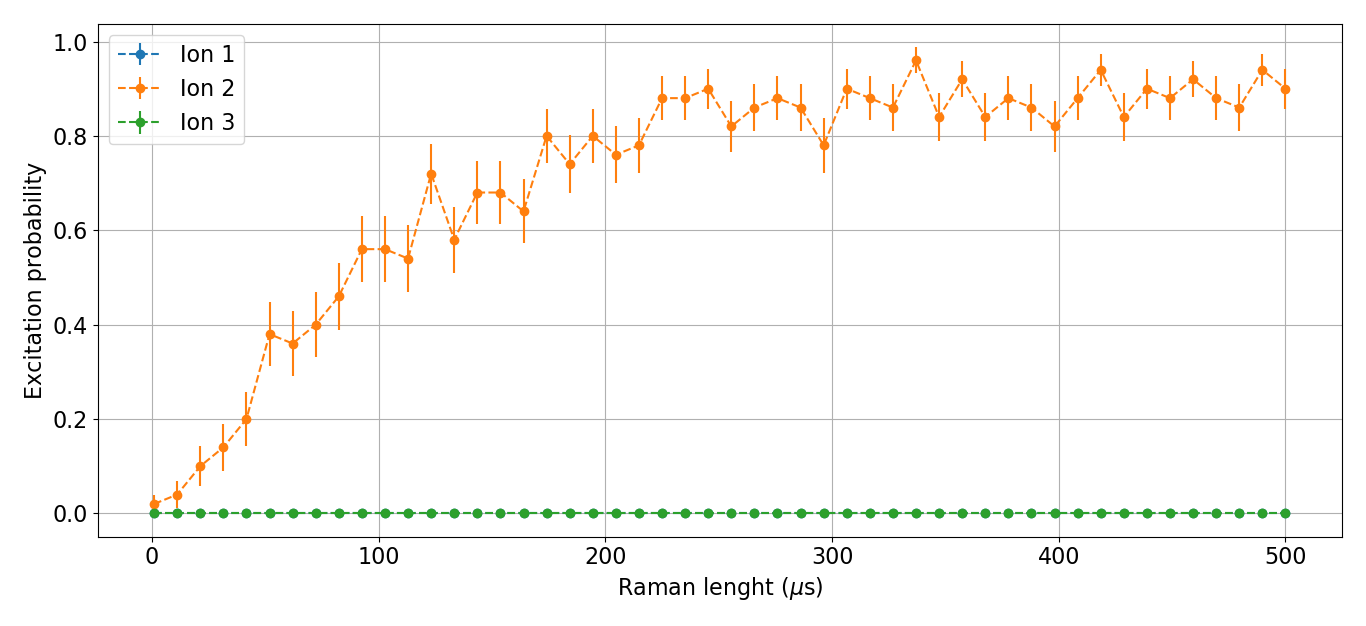
\includegraphics[width=\textwidth]{img/ramanlength_witherrors}
\caption{Qubit state of the ions after sending a Raman pulse.}
\label{probion}
\end{figure}
Errorbars on the excitation probability are calculated as the previous section, while for the photon probability the error is given by Poissonian statistics \cite{quantumoptics}
\begin{equation}
\sigma_{ph} = \frac{\sqrt{N_{click}}}{N},
\end{equation}
where $N_{click}$ is the number of times a photon has been detected with respect to the total $N$ repetitions.
As we can see, only the addressed ion gets excited as emits a photon. The probability of getting photon is relatively low $<15 \%$, as no optimization were performed to increase it.

\section{Final properties summary}
This section contains a summary of the different properties of the setup, everything can be found in the figure below.
\begin{figure}[H]
\centering
\includegraphics[width = \textwidth]{recap}
\caption{Properties summary of the setup.}
\end{figure}
